\chapter{Image Classification Project Lab: Train, Tune, Save and Share}

\begin{glancebox}
You have a dataset; now you will train a model, understand the three settings that control training, tune them by trying, and finally save and share your project. The lab ends with a project you present to friends.
\end{glancebox}

\section*{Learning objectives}

By the end of this chapter you can:


\begin{enumerate}
\item Explain what happens during training and recognize an untrained vs. a trained model.
\item Describe \textbf{epochs}, \textbf{learning rate} and \textbf{batch size}, and what goes wrong when each is too low or too high.
\item Use a train \ensuremath{\rightarrow} test \ensuremath{\rightarrow} retry loop to improve a model, and explain why you test with new pictures.
\item Split your pictures into a training set and a test set.
\item Save a Teachable Machine project and share a model with a link.
\item Build and share a rock-paper-scissors or mask/no-mask classifier.
\end{enumerate}

\section*{Key terms}

\textbf{Training} · \textbf{epoch} · \textbf{learning rate} · \textbf{batch size} · \textbf{overfitting (memorizing)} · \textbf{training set} · \textbf{test set} · \textbf{train-test split} · \textbf{Advanced settings} · \textbf{Preview} · \textbf{export} · \textbf{shareable link}


\section{Recap}

Last chapter you met image types (RGB, grayscale, binary), multi-class classification (can vs. plastic vs. paper), and the idea of \textbf{one folder per class} for storing examples. We now put those folders to work.


\section{What training does}

In Teachable Machine each class holds example images. The workspace shows, for example, three classes (\textbf{Can}, \textbf{Plastic}, \textbf{Paper}) with ten image samples each, and a \textbf{Train Model} button.


\textbf{Before training}, the model is guessing. Show it a picture and the Output bars are close to an even split, roughly a third for each class (the course screenshots show about 31–36\% each). \textbf{After training}, the same kind of picture gets a confident answer. In the course examples a crushed red can went from about 31/38/31\% to \textbf{100\% Can}, a white plastic bottle neck scored \textbf{99\% Plastic}, and crumpled paper scored \textbf{92\% Paper}.


Training means the model looks at your examples over and over, getting better at \emph{predicting the right output}.


Figure \ref{fig:training-before-after} shows example output bars before and after training.


\begin{figure}[htbp]
\centering
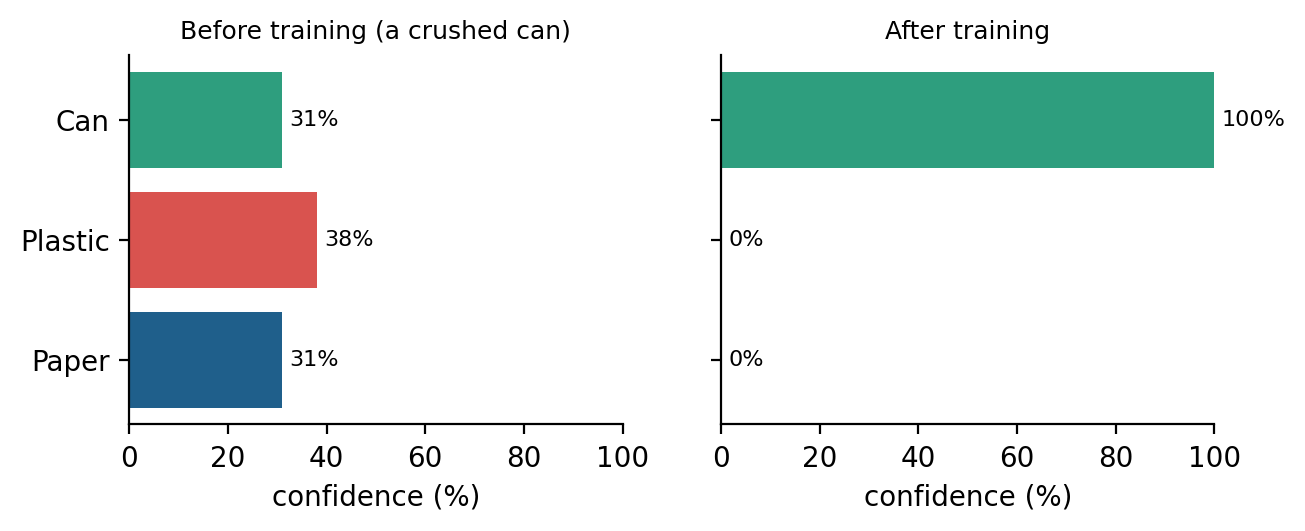
\includegraphics[width=0.9\linewidth]{figures/generated/training-before-after.png}
\caption{Output bars for a crushed-can picture before and after training (example values).}\label{fig:training-before-after}
\end{figure}

\section{Three questions about training}

Training is controlled by three settings in the \textbf{Advanced} panel:


\begin{center}



\renewcommand{\arraystretch}{1.15}

\begin{tabularx}{\linewidth}{>{\raggedright\arraybackslash}X>{\raggedright\arraybackslash}X>{\raggedright\arraybackslash}X}

\toprule

\textbf{Question} & \textbf{Setting} & \textbf{Teachable Machine default} \\

\midrule

How long to train? & \textbf{Epochs} & 50 \\

How large a step to take? & \textbf{Batch size} & 16 \\

How fast to learn? & \textbf{Learning rate} & 0.001 \\

\bottomrule

\end{tabularx}

\end{center}

A \textbf{Reset Defaults} button restores them, and \textbf{Under the hood} shows accuracy per class and a confusion matrix (Chapter 7).


Figure \ref{fig:advanced-panel} shows the Advanced panel with its default values.


\begin{figure}[htbp]
\centering
\adjustbox{max width=\linewidth}{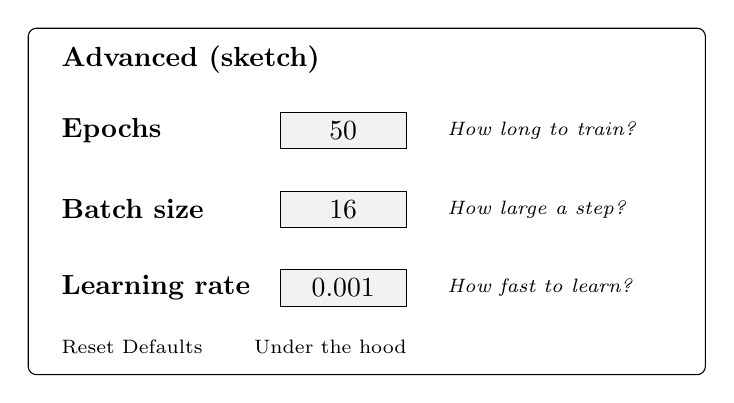
\begin{tikzpicture}[x=1cm,y=1cm]
\draw[rounded corners=3pt,fill=white] (0,0) rectangle (8.6,4.4);
\node[font=\bfseries,anchor=west] at (0.3,4.0) {Advanced (sketch)};
\foreach \y/\n/\v/\q in {3.1/Epochs/50/{How long to train?}, 2.1/Batch size/16/{How large a step?}, 1.1/Learning rate/0.001/{How fast to learn?}}{
 \node[anchor=west] at (0.3,\y) {\textbf{\n}};
 \node[draw,fill=gray!10,minimum width=1.6cm] at (4.0,\y) {\v};
 \node[anchor=west,font=\scriptsize\itshape] at (5.2,\y) {\q};}
\node[font=\scriptsize,anchor=west] at (0.3,0.35) {Reset Defaults \quad\quad Under the hood};
\end{tikzpicture}
}
\caption{The Advanced panel with Teachable Machine’s default values.}\label{fig:advanced-panel}
\end{figure}

\subsection*{Epochs: how long to train}

An \emph{epoch} is one full pass over all your samples.


\begin{itemize}
\item \textbf{Too low (1–5):} not enough time to learn.
\item \textbf{Too high (100–1000):} the model \emph{memorizes} your pictures instead of understanding them. This is called overfitting.
\item \textbf{Solution:} find a good value by trying many times (technically called “tuning”).
\end{itemize}

Figure \ref{fig:epochs-effect} illustrates what too few and too many epochs do.


\begin{figure}[htbp]
\centering
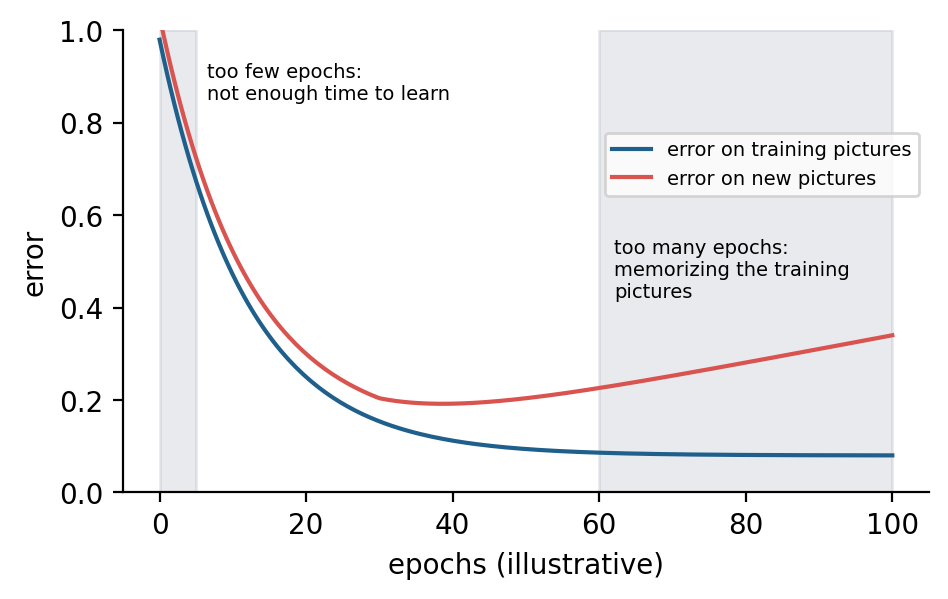
\includegraphics[width=0.7\linewidth]{figures/generated/epochs-effect.png}
\caption{An illustration of the epochs idea: with too few epochs the model has not learned; with too many it memorizes the training pictures and does worse on new ones.}\label{fig:epochs-effect}
\end{figure}

\subsection*{Learning rate: how fast to learn}

The learning rate is how big each adjustment to the model is.


\begin{itemize}
\item \textbf{Too small} (for example 0.000001): learning crawls.
\item \textbf{Too large} (for example 1): the model overshoots and never settles.
\item \textbf{Solution:} again, try values and test.
\end{itemize}

\subsection*{Batch size: how many samples at a time}

The batch size is how many samples the model looks at in each step. Examples shown are 1 and 10. The right choice depends on \textbf{your computer’s computing power}.


\begin{notebox}
\textbf{Go deeper.} Curious what happens inside the model during training? See Appendix C, \emph{How a Model Learns}.
\end{notebox}

\begin{notebox}
\textbf{Teaching note.} The slides picture hand-washing laundry next to a washing machine for this idea; read it as “a few items at a time versus many at once”.
\end{notebox}

\section{The tuning loop}

No single setting is right for every project. Use this loop:


\begin{enumerate}
\item \textbf{Try some settings.}
\item \textbf{Test the model} with new pictures.
\item \textbf{Not OK?} Change a setting (or add better data) and go back to step 1.
\item \textbf{OK?} Done.
\end{enumerate}

Figure \ref{fig:tuning-loop} shows the tuning loop.


\begin{figure}[htbp]
\centering
\adjustbox{max width=\linewidth}{\begin{tikzpicture}[node distance=11mm]
\node[box] (a) {\textbf{1. Try}\\[-1pt]{\scriptsize some settings}};
\node[box,right=of a] (b) {\textbf{2. Test}\\[-1pt]{\scriptsize with new pictures}};
\node[box,right=of b,fill=yellow!20] (c) {\textbf{3. OK?}};
\node[box,right=of c,fill=green!20] (d) {\textbf{Done!}};
\draw[arrow] (a)--(b); \draw[arrow] (b)--(c); \draw[arrow] (c)--node[above,font=\scriptsize]{yes}(d);
\draw[arrow] (c.south)--++(0,-1.0)-|node[pos=0.25,below,font=\scriptsize]{no: change a setting or add data}(a.south);
\end{tikzpicture}
}
\caption{The tuning loop: try, test, and change a setting until the result is acceptable.}\label{fig:tuning-loop}
\end{figure}

\subsection*{Why not test on the training pictures?}

Testing with the same pictures the model trained on is like giving students 100 practice questions to prepare for an exam, and then putting exactly the same 100 questions in the exam. A student who scores 100\% might truly understand the subject, or might simply have \textbf{memorized} the answers. From the scores alone, you cannot tell which.


A model is the same. Pictures it has already seen will almost always get a high score, even if the model has only memorized them (this is the overfitting from the epochs section). To find out whether it has really \textbf{learned} the idea of a can, a plastic bottle or a hand gesture, test it with \textbf{new pictures} it has never seen, like fresh exam questions. \emph{(The exam comparison is the author’s analogy.)}


Testing must use pictures the model has not seen. Compare which hard cases fail, such as a newspaper ad or a clear plastic item, and add varied examples of those classes.


\section{Train-test split}

Section 3.4 said to test with pictures the model has never seen. The easiest way to get such pictures is a \textbf{train-test split}: before you train, divide your pictures for each class into two groups.


\begin{itemize}
\item The \textbf{training set} is what the model learns from.
\item The \textbf{test set} is kept aside. The model never sees it while learning, and you use it \textbf{only} to check the result, like the real exam.
\end{itemize}

A common choice is about \textbf{80\% for training and 20\% for testing}. (This is general practice, not from the slides.) For example, if you have 50 pictures of plastic bottles, put 40 in the training set and keep 10 for testing. Do the same for every class.


Figure \ref{fig:train-test-split} shows the split.


\begin{figure}[htbp]
\centering
\adjustbox{max width=\linewidth}{\begin{tikzpicture}[x=1cm,y=1cm]
\node[font=\bfseries,anchor=west] at (0,3.0) {50 pictures of one class (example)};
\foreach \k in {0,...,39}{\draw[fill=blue!20,draw=blue!50!black] (\k*0.25,2.0) rectangle (\k*0.25+0.2,2.6);}
\foreach \k in {40,...,49}{\draw[fill=orange!35,draw=orange!70!black] (\k*0.25+0.3,2.0) rectangle (\k*0.25+0.5,2.6);}
\node[box,fill=blue!10,minimum width=5.6cm] (tr) at (2.5,0.2) {\textbf{Training set}: 40 pictures (80\%)};
\node[box,fill=orange!15,minimum width=3.4cm] (te) at (9.0,0.2) {\textbf{Test set}: 10 pictures (20\%)};
\draw[arrow] (2.5,1.9)--(tr.north);
\draw[arrow] (9.0,1.9)--(te.north);
\node[box,minimum width=5.6cm] (a) at (2.5,-1.6) {The model \textbf{learns} from these};
\node[box,minimum width=3.4cm] (b) at (9.0,-1.6) {Kept aside; used \textbf{only} to test};
\draw[arrow] (tr.south)--(a.north);
\draw[arrow] (te.south)--(b.north);
\end{tikzpicture}
}
\caption{A train-test split: of 50 pictures of one class, 40 are used for training and 10 are kept aside for testing.}\label{fig:train-test-split}
\end{figure}

\textbf{Rules for a fair split}


\begin{enumerate}
\item \textbf{Split first, then train.} Set the test pictures aside \emph{before} you press Train Model, and never add them to a class.
\item \textbf{Keep the test set untouched.} If a test picture fails, do not copy it into the training set and then re-test with the same picture; take new pictures for the next round of testing.
\item \textbf{Mix the split.} Do not use only the first photos you took for training and the last ones for testing. Pick at random, so both groups contain a mix of angles, light and backgrounds.
\item \textbf{Test every class.} Keep some test pictures for each class, in roughly equal numbers.
\item \textbf{Use other people if you can.} A friend’s photos or handwriting make a tougher, more honest test than your own.
\end{enumerate}

\textbf{How to do it in Teachable Machine.} Keep your test pictures in a separate folder on your computer and do not upload them to any class. After training, test by showing them to the Preview (webcam or \emph{Upload}). Teachable Machine also reports accuracy on its own held-out samples: open \textbf{Advanced \ensuremath{\rightarrow} Under the hood} (see Chapter 7). \emph{(Author’s note: Teachable Machine’s built-in split is not described in the slides; check the exact percentages in the tool before quoting them.)}


Later chapters build on this idea: in Chapter 7 you test with labelled folders of fresh pictures, and in Chapters 8 and 9 you must never augment the test set.


\section{Saving your project}

Saving keeps your work for later. Teachable Machine lets you save \textbf{online} (to Google Drive, or as a shareable link) or \textbf{on your computer} (download the project file). Open the project menu (top left) to find \emph{Save project to Drive} and \emph{Download project as file}. A model link alone cannot be retrained, so save the project itself if you want to add more images.


\section{Sharing your project}

Sharing lets anyone try your model.


\begin{enumerate}
\item Click \textbf{Export Model}.
\item Choose \textbf{Upload (shareable link)}. The export panel also lists TensorFlow.js, TensorFlow and TensorFlow Lite options.
\item Copy the link (it looks like \texttt{teachablemachine.withgoogle.com/models/…}).
\end{enumerate}

Anyone with the link can use the model on their own webcam, so share it with care.


Figure \ref{fig:shared-model-page} shows the page that opens from a shared link: the model’s web address and files on the left, and a live preview on the right where anyone can test the model (here with a picture of a newspaper advertisement, which the model labels Paper).


\begin{figure}[htbp]
\centering
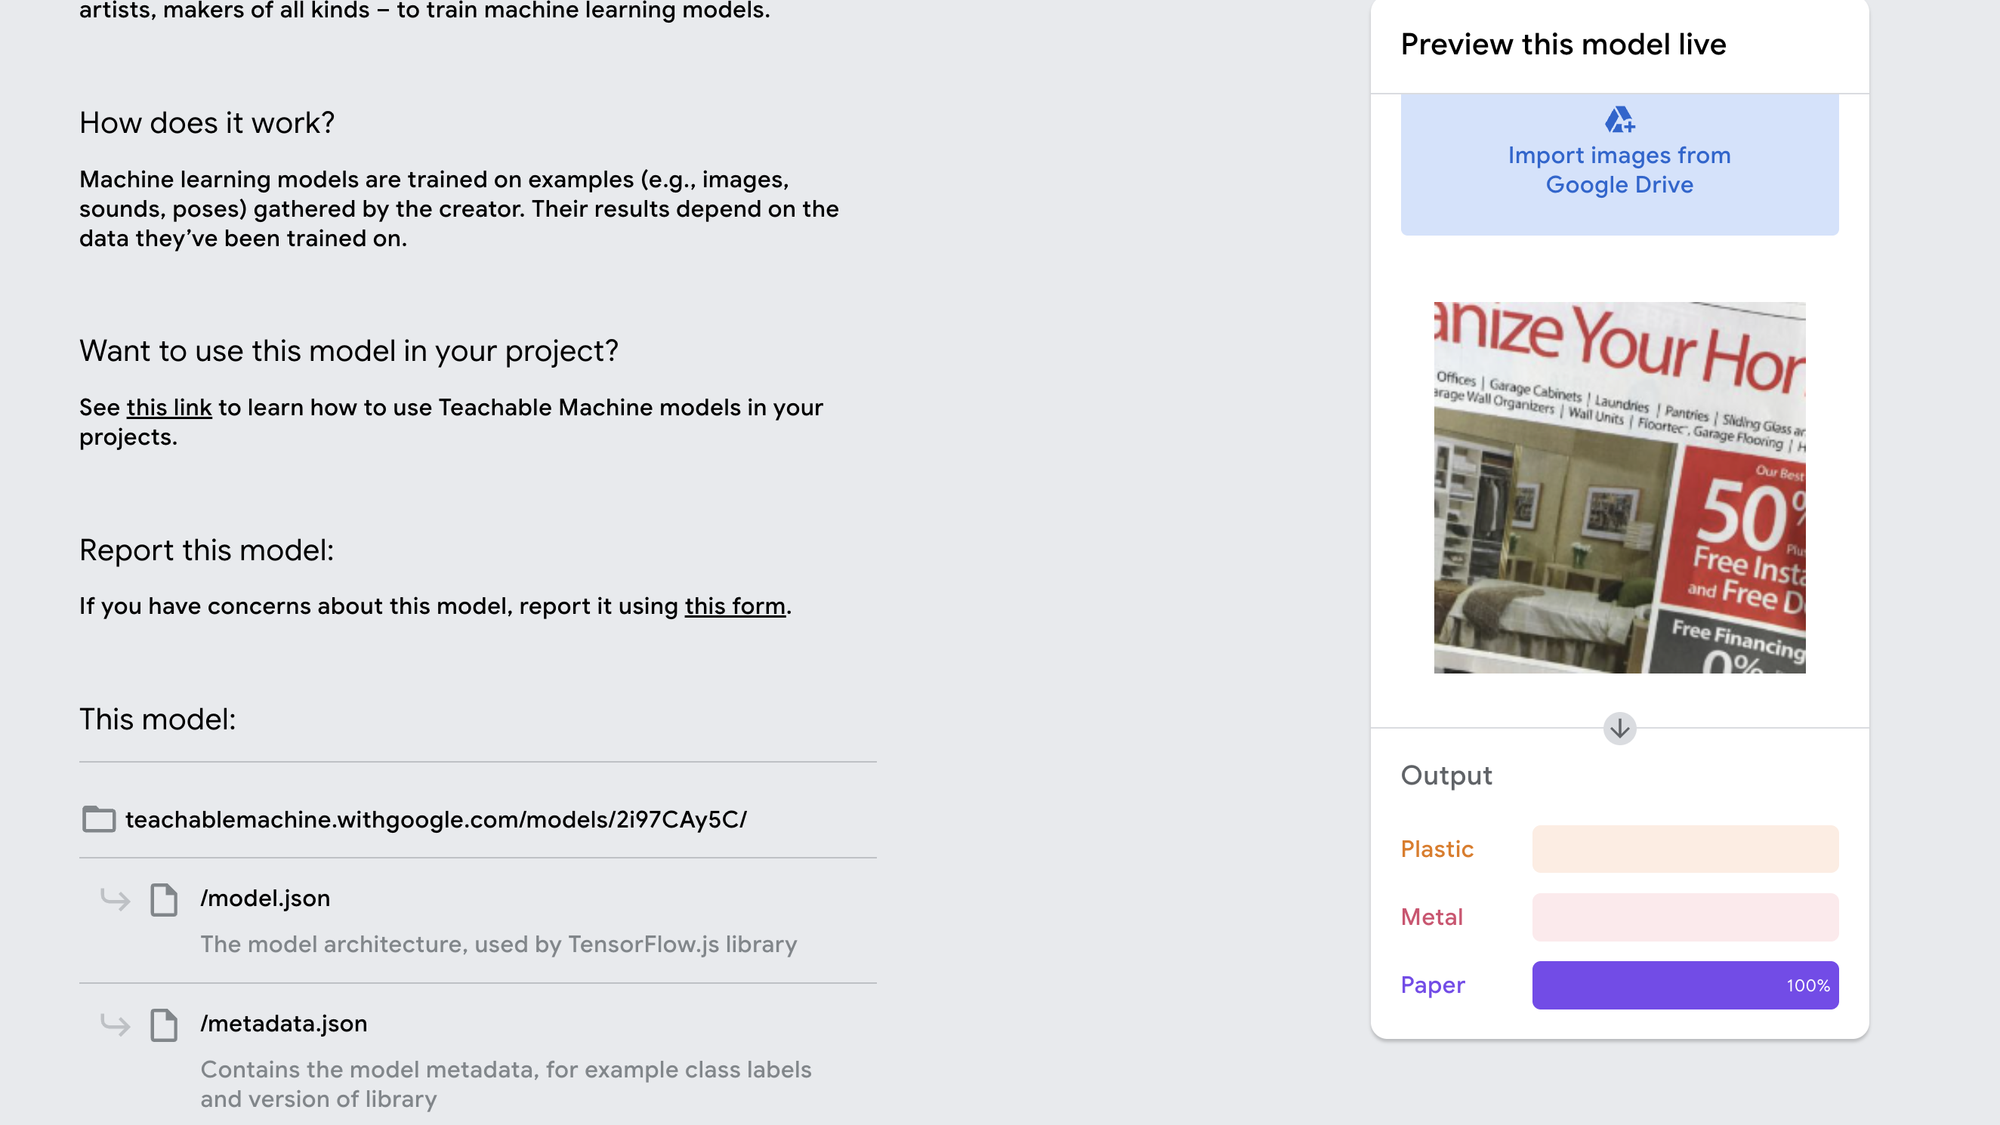
\includegraphics[width=0.95\linewidth]{figures/provided/shared-model-page.png}
\caption{The page for a shared model: its link and files (left) and a live preview with Output bars (right).}\label{fig:shared-model-page}
\end{figure}

\section{Your turn: project lab}

Train \textbf{either} a rock-paper-scissors \textbf{or} a mask / no-mask model:


\begin{enumerate}
\item Create 3 (or 2) classes and collect varied images for each. Keep about 20\% of the pictures aside as a test set.
\item Train with the default settings and test.
\item Tune: try changing epochs, then learning rate or batch size, one at a time.
\item Test with your test set, then with new people and backgrounds.
\item Save the project and share your model link with your instructor or friends.
\end{enumerate}

\section*{Summary}

\begin{itemize}
\item Training makes the model better at predicting the right output; untrained outputs are close to even guesses.
\item Epochs, learning rate and batch size control how long, how fast and how big a step; too much or too little of each causes problems.
\item Improve by looping: try, test, adjust.
\item Split your pictures into a training set (about 80\%) and a test set (about 20\%) before you train, and keep the test set untouched.
\item Test with new pictures, never the training ones: like an exam that repeats the practice questions, a test on training pictures cannot tell understanding from memorizing.
\item Save the project to keep working; share with an exported link.
\end{itemize}

\section*{Check your understanding}

\begin{enumerate}
\item What do the Output bars look like before training?
\item What does a \emph{very high} number of epochs risk?
\item Why change only one setting at a time?
\item What is the difference between saving a project and sharing a model link?
\end{enumerate}

\emph{Answer hints:} (1) near-equal bars. (2) Memorizing instead of understanding. (3) So you know which change caused the result. (4) A project can be retrained; a link only runs the model.


\section*{Further practice}

Record the settings and accuracy for each experiment in a small table, then explain which setting made the biggest difference.


\medskip\noindent\hrulefill\medskip
